\documentclass[a4paper,11pt]{jsarticle}

% パッケージ
\usepackage[dvipdfmx]{hyperref}
\usepackage{pxjahyper}
\usepackage[dvipdfmx]{graphicx}
\usepackage{ascmac}
\usepackage{fancybox}
\usepackage{listings}
\usepackage{plistings}
\usepackage{multirow}
\usepackage[subrefformat=parens]{subcaption}
\usepackage{color}
\usepackage{here}
\usepackage{subcaption}
\usepackage{longtable}
\usepackage{amsmath,amsfonts}
\usepackage[utf8]{inputenc}
\usepackage{bm}
\usepackage{siunitx}
\usepackage{url}
% ページの周りの余白
\usepackage[top=25truemm,bottom=25truemm,left=30truemm,right=30truemm]{geometry}

% URLの設定
\Urlmuskip=0mu  plus 10mu

% 色の定義
\definecolor{OliveGreen}{rgb}{0.0,0.6,0.0}
\definecolor{Magenta}{cmyk}{0, 1, 0, 0}
\definecolor{colFunc}{rgb}{1,0.07,0.54}
\definecolor{CadetBlue}{cmyk}{0.62,0.57,0.23,0}
\definecolor{Brown}{cmyk}{0,0.81,1,0.60}
\definecolor{colID}{rgb}{0.63,0.44,0}


\lstset{
  basicstyle={\ttfamily},
  identifierstyle={\small},
  commentstyle={\smallitshape},
  keywordstyle={\small\bfseries},
  ndkeywordstyle={\small},
  stringstyle={\small\ttfamily},
  frame={tb},
  breaklines=true,
  columns=[l]{fullflexible},
  numbers=left,
  xrightmargin=0zw,
  xleftmargin=3zw,
  numberstyle={\scriptsize},
  stepnumber=1,
  numbersep=1zw,
  lineskip=-0.5ex
}

\renewcommand{\lstlistingname}{Code}

% リンクの設定
\hypersetup{
  setpagesize=false,
  bookmarksnumbered=true,
  bookmarksopen=true,
  colorlinks=true,
  linkcolor=blue,
  citecolor=red,
}

\begin{document}

\section{実験目的}
本実験では,Arduinoを用いた自動ブラインドシステムを構築する.その中でマイコンの割り込み機能
について学習し,割り込み技術を習得することを目的とする.
\section{概要}
\subsection{外部割り込み}
外部割り込み~\cite{interrupt1}とは,外部からの信号で割り込みが発生する仕組みのことである.割り込みが発生すると,CPU
は通常の命令の実行を中断し,割り込みサブルーチンを起動する.割り込みサブルーチンとして準備
されたプロセスが完了すると,元の命令に戻り,途中から実行を再開する.外部割り込みを発生させる
デバイスの例として,マウス.キーボード,スイッチなどが挙げられる.
\subsection{タイマー割り込み}
タイマー割り込み~\cite{interrupt2}とは,設定した時間間隔で割り込みを発生させる仕組みであり,
定期的に発生させたいサブルーチンを呼び出すことができる.割り込みの動作は外部割り込みなどの
ほかの割り込みプロセスと変わらない.

\section{構築したシステム}

\subsection{ハードウェア}
以下の図\ref{P:circuit}に作成した回路を示す.
\begin{figure}[H]
  \centering
  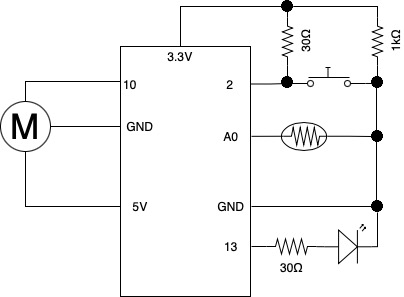
\includegraphics[width=0.7\linewidth]{Circuit.jpg}
  \caption{作成した回路}
  \label{P:circuit}
\end{figure}
Arduino Unoのピン10, GND, 5Vにはサーボモータを接続した.また,ピン13にはLEDとそれに伴う抵抗($30\si{\ohm}$)を接続した.
フォトトランジスタとタクトスイッチにはプルアップ抵抗を接続し,出力状態,センサの状態を反転させている.よって,タクトスイッチを
押したときのみ,ArduinoでONを読み取ることができる.
\subsection{ソフトウェア}
以下のCode\ref{Code}に作成したArduinoのソースコードを示す.
\begin{lstlisting}[caption=Arduinoで作成したCode, label=Code]
#include "Servo.h"
#include "MsTimer2.h"

Servo myservo;
void brind(){
  if(analogRead(A0)<450){
      myservo.write(0); 
  }else if(analogRead(A0)>510){
      myservo.write(180);
  }
}

void setup() {
  Serial.begin(9600);
  pinMode(2, INPUT);
  pinMode(13, OUTPUT);
  
  attachInterrupt(0,interrupt,FALLING);
  
  myservo.attach(10);
  MsTimer2::set(100, brind);
  MsTimer2::start();
}

void loop() {
  digitalWrite(13, HIGH);  
  delay(1000);  
  digitalWrite(13, LOW);
  delay(1000);               
}

void interrupt(){
  Serial.println(analogRead(A0));
}
\end{lstlisting}\par
1行目,2行目ではサーボモータとタイマ割り込みのためのライブラリをインポートしている.
5\ $\sim$ 11行目ではソフトウェア起動時の初期動作を表している.シリアルモニタを起動後,ピン2をフォトレジスタの入力ポートとして割り当て,ピン13を
LEDの出力ポートとして割り当てている.25\ $\sim$ 30行目ではLチカを行う動作を書いている.
18行目にある``attachInterrupt(0, interrupt, FALLING)''は,外部割り込みを命令するコードである.タクトスイッチが押されたとき,
32行目から記している自作のinterrupt関数を動かしている,interrupt関数の中では,シリアルモニタにフォトトランジスタから読み取った明るさの数値
を表示している.また,21,22行目ではタイマ割り込みを命令するコードである.100ms周期で自動的に自作のbrind関数を動かしている.brind関数では,フォトトランジスタ
から読み取った明るさの数値からサーボモータを動かす動作を記している.割り込み動作と,メインのLOOP文を用いることで,バラバラの周期で,自分が指定したタイミング,周期
でプログラムを動作させている.

\section{チャタリングとは}
トグルスイッチや押しボタンスイッチなどの機械式スイッチでは,チャタリング~\cite{chataring}という現象が生じる.チャタリングが生じた際の波形の様子を以下の図\ref{P:chata}に示す.

チャタリングとはスイッチを押したときに接点がピタッと1度で接続されず,バウンド,もしくは擦れが起こることによる現象で,チャタリングが発生時は複数回ON,OFFの切買いが
発生し,最終的にONに落ち着く.
\begin{figure}[H]
  \begin{minipage}{0.48\textwidth}
    \begin{center}
      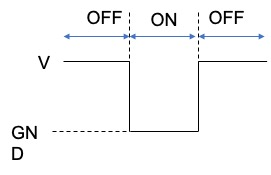
\includegraphics[clip,width=6cm]{picture/chata1.jpg}
    \end{center}
    \subcaption{理想状態のスイッチ}
    \label{chata1}
  \end{minipage}
  \begin{minipage}{0.48\textwidth}
    \begin{center}
      
\includegraphics[clip,width=6cm]{picture/chata2.png}
    \end{center}
    \subcaption{チャタリングが発生しているスイッチ}
    \label{chata2}
  \end{minipage}
  \caption{スイッチによる信号状態p}
  \label{P:chata}
\end{figure}



\begin{thebibliography}{99}
  \bibitem{text} 熊本高等専門学校 制御情報システム工学科授業資料: ``マイコン基礎・応用'' (最終閲覧日 2021年7月6日)\\
  \bibitem{interrupt1} Tech Village: ``ハードウェアの仕組みとソフトウェア処理 ―― マイコンの動作を理解する'' (最終閲覧日 2021年7月6日)\\ \url{http://www.kumikomi.net/archives/2009/11/post_23.php?page=5}\\
  \bibitem{chataring} marutsu: ``スイッチのチャタリングの概要'' (最終閲覧日 2021年7月13日) \\ \url{https://www.marutsu.co.jp/pc/static/large_order/1405_311_ph}
\end{thebibliography}
\end{document}